\documentclass[11pt]{book} % or report
\usepackage{amsmath}
\usepackage{amsfonts}
\usepackage{amssymb}
\usepackage{geometry}
\geometry{a4paper, margin=1in}
\usepackage{graphicx}
\usepackage[hidelinks]{hyperref}
\usepackage{amsthm}
\usepackage{tikz}
\usepackage{subcaption}
\usetikzlibrary{positioning}
\usepackage{pgfplots} 
\usepackage[ruled,vlined]{algorithm2e} 
\usepackage{dsfont}
\usepackage{graphicx}
\usepackage{mathdesign}
\usepackage{float}
\usepackage{todonotes} 
\usepackage{empheq}
\usepackage{array}
\usepackage[ruled,vlined]{algorithm2e} 



\setlength{\parindent}{0pt}

% \let\stdsection\section
% \renewcommand\section{\newpage\stdsection}

\newcommand\mycommfont[1]{\footnotesize\ttfamily\textcolor{blue}{#1}}
\newcommand\defeq{\stackrel{\mathclap{\normalfont\mbox{def}}}{=}}
\SetCommentSty{mycommfont}

\DeclareMathOperator*{\argmax}{argmax}
\DeclareMathOperator*{\argmin}{argmin}

\newtheorem{theorem}{Theorem}[section]
\newtheorem{lemma}{Lemma}[section]
\newtheorem{definition}{Definition}[section]
\newtheorem{corollary}{Corollary}[section]
\newtheorem{claim}{claim}[section]
\newtheorem{example}{Example}[section]


\newtheorem*{claim*}{Claim}
\newtheorem*{lemma*}{Lemma}
\newtheorem*{corollary*}{Corollary}
\newtheorem*{remark*}{Remark}
\newtheorem*{example*}{Example}
\newtheorem*{examples*}{Examples}
\newtheorem*{definition*}{Definition}



\setcounter{tocdepth}{3}





\begin{document}

\begin{titlepage}
    \begin{center}
     {\huge\bfseries 
    Algebra     \\}
     % ----------------------------------------------------------------
     \vspace{1.5cm}
     {\Large\bfseries Hadar Tal}\\[5pt]
     hadar.tal@mail.huji.ac.il\\[14pt]
      % ----------------------------------------------------------------
     \vspace{2cm}
     {This paper is a summary of the educational materials and lectures from 
     \begin{itemize}
        \item \textbf{Wikipedia}
        \item \textbf{3Blue1Brown} YouTube channel
     \end{itemize}
     }

     \vfill
    {Winter 2024}
    \end{center}
\end{titlepage}


\frontmatter
\tableofcontents

% * * * * * * * * * * * * * * * * * * * * * * * * 
% * * * * * * * * * * * * * * * * * * * * * * * * 
% * * * * * * * * * * * * * * * * * * * * * * * * 
% * * * * * * * * * * * * * * * * * * * * * * * * 
% * * * * * * * * * * * * * * * * * * * * * * * * 
% * * * * * * * * * * * * * * * * * * * * * * * * 
% * * * * * * * * * * * * * * * * * * * * * * * * 
% * * * * * * * * * * * * * * * * * * * * * * * * 
% * * * * * * * * * * * * * * * * * * * * * * * * 
% * * * * * * * * * * * * * * * * * * * * * * * * 
% * * * * * * * * * * * * * * * * * * * * * * * * 
% * * * * * * * * * * * * * * * * * * * * * * * * 
% * * * * * * * * * * * * * * * * * * * * * * * * 
% * * * * * * * * * * * * * * * * * * * * * * * * 
% * * * * * * * * * * * * * * * * * * * * * * * * 
% * * * * * * * * * * * * * * * * * * * * * * * * 
% * * * * * * * * * * * * * * * * * * * * * * * * 
% * * * * * * * * * * * * * * * * * * * * * * * * 
% * * * * * * * * * * * * * * * * * * * * * * * * 

\mainmatter
\chapter{Properties}
\begin{definition}{Closure (sgirot) } \\
An operation \(*\) on a set \(G\) is said to have the property of closure if for every \(a, b \in G\), the result \(a * b\) is also in \(G\).
\end{definition}

\begin{definition}{Commutativity (hilofiot)} \\
An operation \(*\) on a set \(G\) is commutative if for every \(a, b \in G\), we have \(a * b = b * a\).
\end{definition}

\begin{definition}{Associativity} \\
An operation \(*\) on a set \(G\) is associative if for every \(a, b, c \in G\), we have \((a * b) * c = a * (b * c)\).
\end{definition}

\begin{definition}{Distributivity} \\
An operation \(*\) on a set \(G\) is distributive if for every \(a, b, c \in G\), we have \(a * (b + c) = a * b + a * c\).
\end{definition}

\begin{definition}{Identity (zehot)} \\
An operation \(*\) on a set \(G\) has an identity element if there exists an element \(e \in G\) such that for every \(a \in G\), \(a * e = e * a = a\).
\end{definition}

\begin{definition}{Inverse (ofchiot)} \\
An operation \(*\) on a set \(G\) has inverses if for every \(a \in G\), there exists an element \(b \in G\) such that \(a * b = b * a = e\), where \(e\) is the identity element.
\end{definition}

\chapter{Algebraic Structures}
\section{Group}
\begin{definition}{\textbf{Group} (havura)} \\
A group is a set \(G\) along with an operation \(*\) such that $\forall a, b, c \in G$ the following properties hold:
\begin {enumerate}
    \item \(a * b \in G\) (closure)
    \item \((a * b) * c = a * (b * c)\) (associativity)
    \item There exists an element \(e \in G\) such that \(a * e = e * a = a\) (identity)
    \item For each \(a \in G\) there exists \(b \in G\) such that \(a * b = b * a = e\) (inverse)
\end{enumerate}
\end{definition}

\begin{example*}
Examples of groups:
\begin{enumerate}
\item \( (\mathbb{R}, +) \) is a group.
\item \( (\mathbb{Z}, +) \) is a group.
\item Non-zero reals, complex, and rational numbers are groups under multiplication.
\end{enumerate}
\end{example*}

\begin{definition}{\textbf{Homomorphism (Groups)}} \\
    Let \( (G, \cdot) \) and \( (H, \ast) \) be groups. A map \( h: G \to H \) is called a homomorphism if it preserves the group operation, meaning that: 
    \begin{equation*}
        \forall g_1, g_2 \in G, \quad h(g_1 \cdot g_2) = h(g_1) \ast h(g_2)
    \end{equation*}
\end{definition}

\begin{example*} Let \( G = (\mathbb{R}, +) \) and \( H = (\mathbb{R}_{>0}, \cdot) \). \\
    The map \( h: \mathbb{R} \to \mathbb{R}_{>0} \) defined by \( h(x) = e^x \) is a homomorphism.
    \begin{align*}
        h(x + y) &= e^{x + y} = e^x \cdot e^y = h(x) \cdot h(y) \\
        h(x \cdot y) &= e^{x \cdot y} = e^x \cdot e^y = h(x) \cdot h(y)
    \end{align*}
\end{example*}


\begin{definition}{\textbf{Abelian Group}} \\
    An abelian group is a group \( (G, *) \) in which the binary operation \( * \) is commutative, 
    meaning that for all \(a, b \in G\), \(a * b = b * a\).
\end{definition}

\section{Ring}

\begin{definition}{\textbf{Ring} (hug)} \\
    A ring is a set \(R\) equipped with two binary operations \(+\) (addition) and \(\times\) (multiplication) satisfying the following three sets of axioms:
    \begin{enumerate}
        \item \(R\) is an \textbf{abelian group} under addition, meaning that:
        \begin{itemize}
            \item \((a + b) + c = a + (b + c)\) for all \(a, b, c \in R\) (associativity).
            \item \(a + b = b + a\) for all \(a, b \in R\) (commutativity).
            \item There is an element \(0 \in R\) such that \(a + 0 = a\) for all \(a \in R\) (additive identity).
            \item For each \(a \in R\) there exists \(-a \in R\) such that \(a + (-a) = 0\) (additive inverse).
        \end{itemize}
        \item \(R\) is a \textbf{monoid} under multiplication, meaning that:
        \begin{itemize}
            \item \((a \times b) \times c = a \times (b \times c)\) for all \(a, b, c \in R\) (associativity).
            \item There is an element \(1 \in R\) such that \(a \times 1 = a\) and \(1 \times a = a\) for all \(a \in R\) (multiplicative identity).
        \end{itemize}
        \item Multiplication is distributive with respect to addition, meaning that:
        \begin{itemize}
            \item \(a \times (b + c) = (a \times b) + (a \times c)\) for all \(a, b, c \in R\) (left distributivity).
            \item \((b + c) \times a = (b \times a) + (c \times a)\) for all \(a, b, c \in R\) (right distributivity).
        \end{itemize}
    \end{enumerate}

\end{definition}

\begin{example*}
Examples of rings:
\begin{enumerate}
\item \( (\mathbb{Z}, +, \times) \) is a ring.
\item \( (\mathbb{R}, +, \times) \) is a ring.
\item The set of odd integers is not a ring because it is not closed under addition.
\end{enumerate}
\end{example*}

\section{Field}
\begin{definition}{\textbf{Field} (sadeh)} \\
    A field is a set \(F\) with two operations, addition \(+\) and multiplication \(\times\), such that:
    \begin{enumerate}
        \item \( (F, +) \) is an \textbf{abelian group} with the identity element \(0\) (additive identity).
        \item \( (F \setminus \{0\}, \times) \) is an \textbf{abelian group} with the identity element \(1\) (multiplicative identity).
        \item Multiplication is distributive with respect to addition, meaning that:
        \begin{itemize}
            \item \(a \times (b + c) = (a \times b) + (a \times c)\) for all \(a, b, c \in R\) (left distributivity).
            \item \((b + c) \times a = (b \times a) + (c \times a)\) for all \(a, b, c \in R\) (right distributivity).
        \end{itemize}
    \end{enumerate}
\end{definition}

\begin{example*}
Examples of fields:
\begin{enumerate}
\item \( (\mathbb{R}, +, \times) \) is a field.
\item \( (\mathbb{Q}, +, \times) \) is a field.
\item \( (\mathbb{C}, +, \times) \) is a field.
\item \( (\mathbb{Z}_p, +, \times) \) for a prime \(p\) is a field.
\end{enumerate}
\end{example*}

\begin{figure}
    \centering
    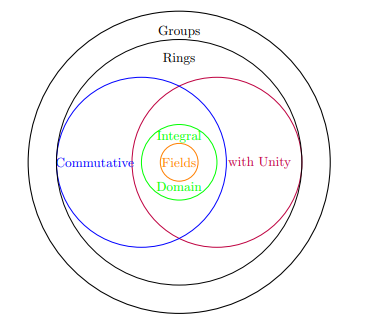
\includegraphics[width=0.5\textwidth]{Figs/algebric_structures.png}
    \caption{Algebraic Structures}
\end{figure}

\chapter{Vector Space}

A major difference between a field and a vector space is that the operations on a field \( \mathbb{F} \) are
\begin{itemize}
    \item \( +: \mathbb{F} \times \mathbb{F} \to \mathbb{F} \)
    \item \( \times: \mathbb{F} \times \mathbb{F} \to \mathbb{F} \)
\end{itemize}

but the operations on a vector space \( \mathbb{V} \) over a field \( \mathbb{F} \) are
\begin{itemize}
    \item \( +: \mathbb{V} \times \mathbb{V} \to \mathbb{V} \)
    \item \( \cdot: \mathbb{F} \times \mathbb{V} \to \mathbb{V} \)
\end{itemize}

\bigbreak

\begin{definition}{\textbf{Vector Space}} \\
    A vector space over a field \( F \) is a non-empty set \( V \) together with two operations: vector addition \( + \) and scalar multiplication \( \cdot \), satisfying the following axioms for every \( u, v, w \in V \) and \( a, b \in F \):
    \begin{enumerate}
        \item Associativity of vector addition: \( u + (v + w) = (u + v) + w \)
        \item Commutativity of vector addition: \( u + v = v + u \)
        \item Identity element of vector addition: There exists an element \( 0 \in V \), called the \textbf{zero vector}, such that \( v + 0 = v \) for all \( v \in V \).
        \item Inverse elements of vector addition: For every \( v \in V \), there exists an element \( -v \in V \), called the \textbf{additive inverse} of \( v \), such that \( v + (-v) = 0 \).
        \item Compatibility of scalar multiplication with field multiplication: \( a(bv) = (ab)v \)
        \item Identity element of scalar multiplication: \( 1v = v \), where \( 1 \) denotes the multiplicative identity in \( F \).
        \item Distributivity of scalar multiplication with respect to vector addition: \( a(u + v) = au + av \)
        \item Distributivity of scalar multiplication with respect to field addition: \( (a + b)v = av + bv \)
    \end{enumerate}
\end{definition}

\begin{example*}
Examples of vector spaces:
\begin{enumerate}
\item \( \mathbb{R}^n \) is a vector space.
\item The space \( M_{m \times n}(\mathbb{F}) \) of \( m \times n \) matrices over a field \(\mathbb{F}\) is a vector space.
\item The set of all continuous functions over some interval is a vector space.
\item The space of all differentiable functions over a certain interval is a vector space.
\end{enumerate}
\end{example*}

\begin{definition}{\textbf{Homomorphism (Vector spaces)}} \\
    Let \(V\) and \(W\) be vector spaces over the same field \(F\). A map \( T: V \to W \) is called a \textbf{homomorphism}, 
    or more specifically, a \textbf{linear transformation}, if for all vectors \(u, v \in V\) and any scalar \(c \in F\), the following conditions hold:
    \begin{itemize}
        \item \textbf{Additivity:} \( T(u + v) = T(u) + T(v) \).
        \item \textbf{Homogeneity:} \( T(c \cdot u) = c \cdot T(u) \).
    \end{itemize}
    These conditions ensure that the map \(T\) preserves the vector space structure between \(V\) and \(W\).
\end{definition}

\begin{definition}{\textbf{Image and Kernel}} \\
    Let \( V \) and \( W \) be vector spaces over a field \( F \), and let \( T: V \to W \) be a linear transformation.  \\
    The \textbf{image} of \( T \), denoted \( \text{Im}(T) \), is the set of all vectors in \( W \) that can be expressed as \( T(v) \) for some \( v \in V \). \\
    The \textbf{kernel} of \( T \), denoted \( \text{Ker}(T) \), is the set of all vectors in \( V \) that are mapped to the zero vector in \( W \), i.e., \( T(v) = 0 \).
\end{definition}


If a homomorphism is bijective, it is called an isomorphism.

\begin{definition}{\textbf{Isomorphism (Vector spaces)}} \\
    Let \( V \) and \( W \) be vector spaces over the same field \( F \). 
    A map \( T: V \to W \) is called an \textbf{isomorphism} if it is a bijective \textbf{linear transformation}, 
    meaning that \( T \) is both a homomorphism and has an inverse \( T^{-1}: W \to V \) which is also a homomorphism. 
    For \( T \) to be an isomorphism, the following conditions must be met:
    \begin{itemize}
        \item \textbf{Bijectivity:} \( T \) is one-to-one and onto.
        \item \textbf{Additivity:} \( T(u + v) = T(u) + T(v) \) for all vectors \( u, v \in V \).
        \item \textbf{Homogeneity:} \( T(c \cdot u) = c \cdot T(u) \) for all vectors \( u \in V \) and any scalar \( c \in F \).
    \end{itemize}
    An isomorphism thus establishes a perfect correspondence between the two vector spaces, preserving all vector space operations.
\end{definition}

If \(V\) and \(W\) are isomorphic, we write \(V \cong W\).


\begin{definition}{\textbf{Complex conjugate}} \\
    The complex conjugate of a complex number \( z = a + bi \) is the number \( \overline{z} = a - bi \).
\end{definition}

\section{Basis and Dimension}

\begin{definition}{\textbf{Basis}} \\
    Let \( V \) be a vector space over a field \( F \). A set of vectors \( \{v_1, v_2, \dots, v_n\} \) in \( V \) is called a basis of \( V \) if every vector \( v \in V \) can be expressed as a unique linear combination of the basis vectors:
    \[
    v = \sum_{i=1}^n a_i v_i
    \]
    where \( a_i \in F \) are scalars. The basis vectors must be linearly independent, meaning that no vector in the set can be expressed as a linear combination of the others.
\end{definition}

\begin{definition}{\textbf{Dimension}} \\
    The dimension of a vector space \( V \) is the number of vectors in any basis of \( V \). The dimension of \( V \) is denoted \( \text{dim}(V) \).
\end{definition}

\begin{definition}{\textbf{Rank}} \\
    The rank of a matrix is the dimension of the vector space spanned by its columns.
\end{definition}

\begin{definition}{\textbf{Nullity}} \\
    The nullity of a matrix is the dimension of the vector space of solutions to the homogeneous system \( Ax = 0 \).
\end{definition}

\begin{definition}{\textbf{Rank-Nullity Theorem}} \\
    Let \( A \) be an \( m \times n \) matrix. The rank of \( A \) plus the nullity of \( A \) equals the number of columns in \( A \), i.e., 
    \[
    \text{rank}(A) + \text{nullity}(A) = n
    \]
\end{definition}

\begin{definition}{\textbf{Invertible matrix}} \\
    A square matrix \( A \) is invertible if there exists a matrix \( A^{-1} \) such that \( A A^{-1} = A^{-1} A = I \), where \( I \) is the identity matrix.
\end{definition}

\section{Cross Product and The determinant}

\begin{definition}{\textbf{Determinant}} \\
    The determinant of a square matrix \( A \) is a scalar value that is computed from the elements of \( A \) and provides significant information about the matrix.     
    For a \( 2 \times 2 \) matrix 
    \[
    det(A) = det( \begin{bmatrix} a & b \\ c & d \end{bmatrix} ) = ad - bc
    \]
    For an \( n \times n \) matrix \( A \), the determinant can be calculated using Laplace's expansion, which is defined as:
    \[
    \det(A) = \sum_{j=1}^{n} (-1)^{i+j} a_{ij} \det(A_{ij}) = \sum_{\sigma \in S_n} \text{sgn}(\sigma) \prod_{i=1}^{n} a_{i, \sigma(i)}
    \]
    where 
    \begin{itemize}
        \item \( a_{ij} \) is the element at the \( i \)-th row and \( j \)-th column of \( A \).
        \item \( A_{ij} \) is the \((n-1) \times (n-1)\) matrix obtained by removing the \( i \)-th row and \( j \)-th column from \( A \).
        \item \( S_n \) is the set of all permutations of \( n \) elements.
        \item \( \text{sgn}(\sigma) \) is the sign of the permutation \( \sigma \), which is \( +1 \) if \( \sigma \) is even and \( -1 \) if \( \sigma \) is odd.
    \end{itemize}
\end{definition}

\paragraph{Intuition for the Determinant} : \\
The determinant of a matrix can be thought of as a measure of the volume scaling factor by which a linear transformation affects a given volume when applied to a space. 
If the determinant is zero, the transformation compresses the space into a lower dimension, leading to a loss in volume. 
If the determinant is positive, the orientation of the space is preserved after transformation; if negative, the orientation is reversed.


\begin{figure}[H]
    \begin{subfigure}{0.4\textwidth}
        \centering
        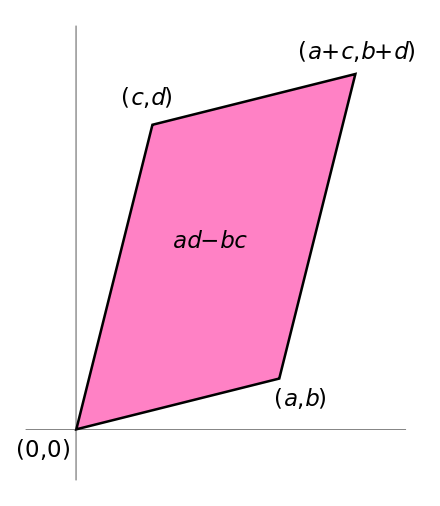
\includegraphics[width=0.8\textwidth]{Figs/area_parallellogram_as_determinant.png}
        \caption{The area of the parallelogram is the absolute value of the determinant of the matrix formed by the vectors representing the parallelogram's sides.}
    \end{subfigure}
    \hfill
    \begin{subfigure}{0.4\textwidth}
        \centering
        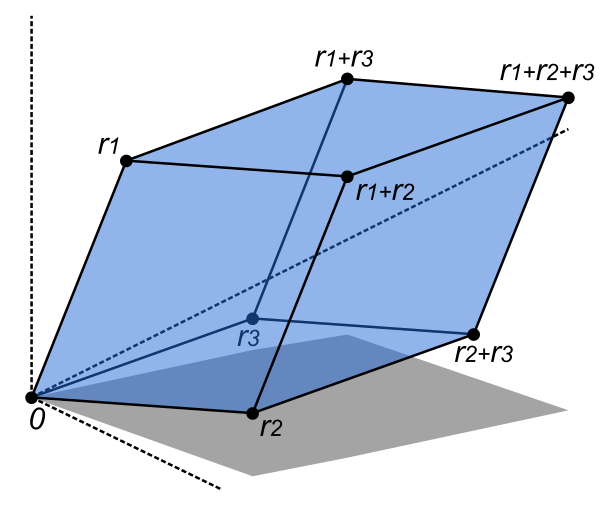
\includegraphics[width=0.8\textwidth]{Figs/determinant_parallelepiped.png}
        \caption{The volume of this parallelepiped is the absolute value of the determinant of the matrix formed by the columns constructed from the vectors r1, r2, and r3.}
    \end{subfigure}
\end{figure}

\begin{definition}{\textbf{Cross Product (in $\mathbb{R}^3$)}} \\
    The cross product of two vectors \( u = (u_1, u_2, u_3) \) and \( v = (v_1, v_2, v_3) \) in \( \mathbb{R}^3 \) is a vector \( u \times v \) defined as:
    \[
    u \times v = \begin{bmatrix} i & j & k \\ u_1 & u_2 & u_3 \\ v_1 & v_2 & v_3 \end{bmatrix} = (u_2 v_3 - u_3 v_2) i - (u_1 v_3 - u_3 v_1) j + (u_1 v_2 - u_2 v_1) k
    \]
\end{definition}

Let \( u = (x_1, y_1, z_1) \) and \( v = (x_2, y_2, z_2) \) be two vectors in \( \mathbb{R}^3 \). 
The cross product of \( u \) and \( v \) is orthogonal to both \( u \) and \( v \), and its magnitude is equal to the area of the parallelogram spanned by \( u \) and \( v \).
\begin{proof}
    We will define new axis: 
    \begin{itemize}
        \item i-axis: will be the span of \( u \)
        \item j-axis: will be orthogonal to the x-axis such that \( y \in span({u, v}) \)
        \item k-axis: will be orthogonal to the x and y axes
    \end{itemize}
    Then, we can write \( u \) and \( v \) as:
    \begin{align*}
        u &= \begin{pmatrix}x1 \\ 0 \\ 0\end{pmatrix} \quad v = \begin{pmatrix}x2 \\ y2 \\ 0\end{pmatrix} \\
        u \times v &= det\begin{pmatrix}i & j & k \\ x1 & 0 & 0 \\ x2 & y2 & 0\end{pmatrix} = 
         0 i - 0 j + x1 \cdot y2 \cdot k = \begin{pmatrix}0 \\ 0 \\ x1 \cdot y2\end{pmatrix} \\
         | \vec{w} | &= | \vec{u} | \times | \vec{v} | = | x1 \cdot y2 | = | x1 | \times | y2 | = \text{area of the parallelogram}
    \end{align*}
\end{proof}

\begin{figure}[H]
    \centering
    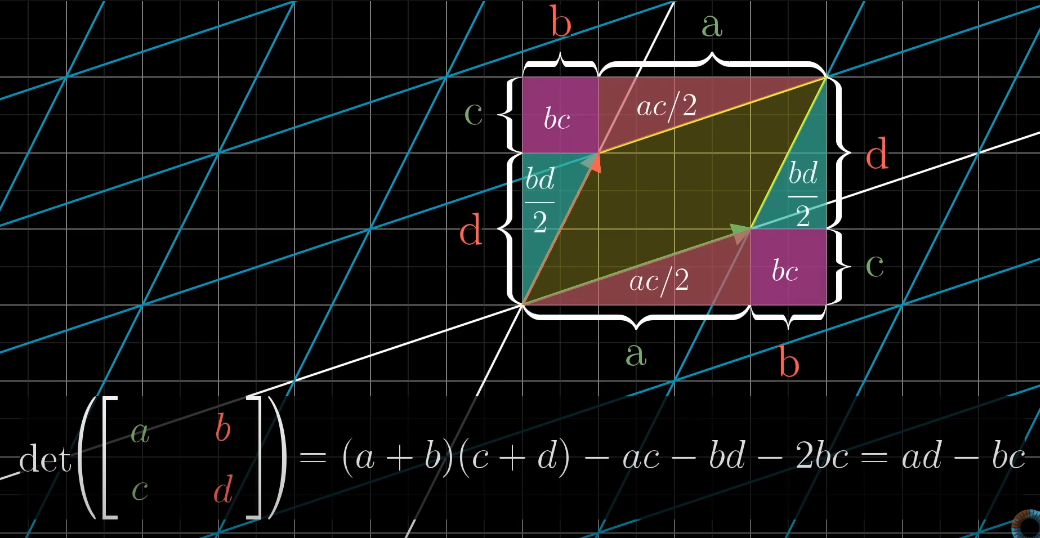
\includegraphics[width=0.7\textwidth]{Figs/determinant_in_R2.png}
    \caption{The determinant of a \( 2 \times 2 \) matrix is the area of the parallelogram spanned by the column vectors.}
\end{figure}

\begin{definition}{\textbf{Cross Product (in $\mathbb{R}^n$)}} \\
    The cross product of two vectors \( u \) and \( v \) in \( \mathbb{R}^n \) is a vector \( u \times v \) defined as:
    \[
    u \times v = \text{det} \begin{bmatrix} e_1 & e_2 & \dots & e_n \\ u_1 & u_2 & \dots & u_n \\ v_1 & v_2 & \dots & v_n \end{bmatrix}
    \]
\end{definition}

\begin{theorem}
Let \( A \) be an \( n \times n \) matrix. The following statements are equivalent:
\begin{enumerate}
    \item The matrix \( A \) is invertible.
    \item The determinant of \( A \) is nonzero (\( \det(A) \neq 0 \)).
    \item The rank of \( A \) is \( n \).
    \item \( A \) can be expressed as a product of elementary matrices.
    \item The dimension of the column space of \( A \) is \( n \).
\end{enumerate}
\end{theorem}

\begin{proof}
The equivalence of these conditions results from fundamental principles in linear algebra:
\begin{itemize}
    \item A non-zero determinant implies that the linear transformation associated with \( A \) is volume preserving and thus has no zero eigenvalues, which implies invertibility.
    \item An invertible matrix has full rank (\( n \)), meaning every row and column contributes to the matrix's span, ensuring that the transformation is onto and one-to-one.
    \item A matrix with full rank \( n \) means there are no free variables in its row-reduced form, hence it transforms \( \mathbb{R}^n \) onto itself without reducing dimension, corroborating the property of invertibility.
    \item The ability to express \( A \) as a product of elementary matrices indicates a series of elementary row operations that transform \( I \) to \( A \), again confirming the full rank and invertibility of \( A \).
\end{itemize}
\end{proof}

\todo[inline]{Add stuff about Leibniz formula for determinant}

% * * * * * * * * * * * * * * * * * * * * * * * *
% * * * * * * * * * * * * * * * * * * * * * * * *
% * * * * * * * * * * * * * * * * * * * * * * * *
% * * * * * * * * * * * * * * * * * * * * * * * *
% * * * * * * * * * * * * * * * * * * * * * * * *
% * * * * * * * * * * * * * * * * * * * * * * * *
% * * * * * * * * * * * * * * * * * * * * * * * *

\section{Eigenvalues and Eigenvectors}


\begin{definition}{\textbf{Conjugate transpose}} \\
    The conjugate transpose of a matrix \( A \) is the matrix obtained by taking the transpose of \( A \) and then taking the complex conjugate of each entry.
\end{definition}

\begin{example}
    Consider the matrix 
    \[
    A = \begin{bmatrix} 1+i & 2-i \\ 3+i & 4-2i \end{bmatrix}.
    \]
    The conjugate transpose of \( A \), denoted \( A^* \) or \( A^\dagger \), is calculated by first transposing the matrix, and then taking the complex conjugate of each element. Thus,
    \[
    A^* = \begin{bmatrix} 1-i & 3-i \\ 2+i & 4+2i \end{bmatrix}.
    \]
\end{example}

\begin{definition}{\textbf{Unitary matrix}} \\
    A square matrix \( U \) is called unitary if its conjugate transpose is equal to its inverse, i.e., \( U^* U = U U^* = I \).
\end{definition}

\begin{definition}{\textbf{Orthogonal complement}} \\
    Let \( V \) be a vector space over a field \( F \) and \( W \) be a subspace of \( V \). The orthogonal complement of \( W \), denoted \( W^\perp \), 
    is the set of all vectors in \( V \) that are orthogonal to every vector in \( W \).
\end{definition}

\begin{definition}{\textbf{Similarity}} \\
    Two matrices \( A \) and \( B \) are said to be similar if there exists an invertible matrix \( P \) such that \( B = P^{-1} A P \).
\end{definition}

\begin{definition}{\textbf{Diagonalizable}} \\
    A matrix \( A \) is said to be diagonalizable if it is similar to a diagonal matrix, i.e., 
    if there exists an invertible matrix \( P \) such that \( P^{-1} A P = D \), where \( D \) is a diagonal matrix.
\end{definition}

\begin{definition}{\textbf{Eigenvalue and Eigenvector}} \\
    Let \( A \) be an \( n \times n \) matrix. A scalar \( \lambda \) is called an eigenvalue of \( A \) if there exists a non-zero vector \( v \) such that \( A v = \lambda v \). 
    The vector \( v \) is called an eigenvector corresponding to the eigenvalue \( \lambda \).
\end{definition}

\begin{definition}{\textbf{Characteristic polynomial}} \\
    The characteristic polynomial of a square matrix \( A \) is defined as \( \text{det}(A - \lambda I) \), where \( I \) is the identity matrix.
\end{definition}

\begin{definition}{\textbf{Cayley-Hamilton Theorem}} \\
    Let \( A \) be an \( n \times n \) matrix. The Cayley-Hamilton theorem states that the matrix \( A \) satisfies its own characteristic equation, i.e., 
    \( p(A) = 0 \), where \( p(\lambda) \) is the characteristic polynomial of \( A \).
\end{definition}

\begin{definition}{\textbf{Spectral decomposition}} \\
    The spectral decomposition of a matrix \( A \) is a representation of \( A \) as a sum of its eigenvectors and eigenvalues, i.e., 
    \( A = PDP^{-1} \), where \( P \) is the matrix whose columns are the eigenvectors of \( A \) and \( D \) is the diagonal matrix of eigenvalues.
\end{definition}

\begin{definition}{\textbf{Unitary diagonalization}} \\
    A matrix \( A \) is said to be unitarily diagonalizable if it is similar to a diagonal matrix by a unitary matrix, i.e., 
    if there exists a unitary matrix \( U \) such that \( U^* A U = D \), where \( D \) is a diagonal matrix.
\end{definition}

\begin{theorem}
    Let \( A \) be an \( n \times n \) matrix. The following statements are equivalent:
    \begin{enumerate}
        \item The matrix \( A \) is unitarily diagonalizable.
        \item The matrix \( A \) is normal, i.e., \( A^* A = A A^* \).
        \item The matrix \( A \) has an orthonormal basis of eigenvectors.
    \end{enumerate}
\end{theorem} 

% * * * * * * * * * * * * * * * * * * * * * * * *
% * * * * * * * * * * * * * * * * * * * * * * * *
% * * * * * * * * * * * * * * * * * * * * * * * *
% * * * * * * * * * * * * * * * * * * * * * * * *
% * * * * * * * * * * * * * * * * * * * * * * * *
% * * * * * * * * * * * * * * * * * * * * * * * *
% * * * * * * * * * * * * * * * * * * * * * * * *


\section{Quadradic and Bilinear Forms}

\begin{definition}{\textbf{Congruence}} \\
    Two matrices \( A \) and \( B \) are said to be congruent if there exists an invertible matrix \( P \) such that \( B = P^T A P \).
\end{definition}


\begin{definition}{\textbf{Quadratic Form}} \\
    A quadratic form on a vector space \( V \) over a field \( F \) is a function \( Q: V \to F \) that is homogeneous of degree 2, 
    meaning that for all \( v \in V \) and \( a \in F \), the quadratic form satisfies:
    \begin{enumerate}
        \item Homogeneity: \( Q(av) = a^2 Q(v) \)
        \item Additivity: \( Q(u + v) = Q(u) + Q(v) \)
    \end{enumerate}
\end{definition}

Any $n \times n$ matrix $A$ defines a quadratic form $Q(v) = v^T A v$ for $v \in \mathbb{R}^n$.  \\
Two matrices $A$ and $B$ define the same quadratic form if and only if they have the same elements on the diagonal and $a_{ij} + a_{ji} = b_{ij} + b_{ji}$ for all $i \neq j$. \\
In general a quadratic form can be written as $Q(v) = v^T A v$ where $A$ is a symmetric matrix. \\
The correspondence between quadratic forms and symmetric matrices is one-to-one, when the basis is fixed.

\begin{definition}{\textbf{Bilinear Form}}
    A bilinear form on a vector space \( V \) over a field \( F \) is a function \( B: V \times V \to F \) that is linear in each of its two arguments independently. This means that for all \( u, v, w \in V \) and \( a \in F \), the bilinear form satisfies:
    \begin{enumerate}
        \item Linearity in the first argument: \( B(au + w, v) = a B(u, v) + B(w, v) \)
        \item Linearity in the second argument: \( B(u, av + w) = a B(u, v) + B(u, w) \)
    \end{enumerate}
    The bilinear form \( B \) is symmetric if \( B(u, v) = B(v, u) \) for all \( u, v \in V \).
\end{definition}

\paragraph{Matrix Representation of a Bilinear Form}: \\ 
Every bilinear form \( B \) on a finite-dimensional vector space \( V \) can be represented by a matrix \( A \) with respect to a basis 
\( \{e_1, e_2, \dots, e_n\} \) of \( V \). 
The entry \( a_{ij} \) in the matrix is defined as \( a_{ij} = B(e_i, e_j) \). Thus, the matrix \( A \) of the bilinear form \( B \) is given by:
\[
A = [a_{ij}] \quad \text{where} \quad a_{ij} = B(e_i, e_j)
\]
Let \( u = \sum_{i=1}^n u_i e_i \) and \( v = \sum_{j=1}^n v_j e_j \) be vectors in \( V \). The matrix representation of the bilinear form \( B \) is then:
\[
B(u, v) = u^T A v 
= \begin{bmatrix} u_1 & u_2 & \cdots & u_n \end{bmatrix} \begin{bmatrix} a_{11} & a_{12} & \cdots & a_{1n} \\ a_{21} & a_{22} & \cdots & a_{2n} \\ \vdots & \vdots & \ddots & \vdots \\ a_{n1} & a_{n2} & \cdots & a_{nn} \end{bmatrix} \begin{bmatrix} v_1 \\ v_2 \\ \vdots \\ v_n \end{bmatrix}
= \sum_{i=1}^n \sum_{j=1}^n a_{ij} u_i v_j
\]


\begin{theorem}{:} \\
    Two matrices \( A \) and \( B \) are congruent if and only if they represent the same quadratic (bilinear) form, i.e., \( Q_A(v) = Q_B(v) \) for all \( v \).
\end{theorem}

\begin{proof} 
    Let $v_1, v_2, \ldots, v_n$ be some basis in $\mathbb{R}^n$, and consider the matrix $P$ whose columns are these basis vectors. 
    Then $P$ is non singular and $\forall x \in \mathbb{R}^n$, $\exists y \in \mathbb{R}^n$ such that $x = Py$. \\
    \\
    Let \( A \) and \( B \) be congruent matrices, i.e., \( B = P^T A P \) for some invertible matrix \( P \). 
    Then, for any vector \( v \), we have:
    \[
    Q_B(v) = v^T B v = v^T P^T A P v = (Pv)^T A (Pv) 
    \]
    Thus, the quadratic form \( Q_B(v) \) is represented by the matrix \( A \) in the basis \( Pv \). 
\end{proof}


\paragraph{Differences Between Congruence and Similarity}: \\

While both congruence and similarity involve transformations of matrices via invertible matrices, they are used in different contexts and have distinct algebraic implications:

\begin{itemize}
    \item \textbf{Congruence}: This relationship focuses on the geometric properties of matrices, 
    particularly those representing quadratic forms or symmetric bilinear forms. When two matrices \( A \) and \( B \) are congruent, 
    it implies that they represent the same quadratic form but in possibly different coordinate systems. 
    The transformation \( B = P^T A P \) can be interpreted as a change of basis in which the basis vectors are orthogonalized or rotated, 
    maintaining the essence of the geometric structure represented by the matrix. 
    Thus, congruence preserves the type of conic sections (e.g., ellipses, hyperbolas) or other geometric objects described by these forms under orthogonal transformations.

    \item \textbf{Similarity}: Similarity transformations are concerned with the preservation of eigenvalues of a matrix. 
    When \( A \) and \( B \) are similar, they represent the same linear transformation expressed in different bases. 
    The condition \( B = P^{-1} A P \) indicates that changing the basis does not alter the intrinsic properties of the linear transformation such as 
    trace, determinant, and eigenvalues. Essentially, similarity is related to the fundamental operations of the matrix and does not 
    concern itself directly with geometric interpretations in the same way as congruence. 

\end{itemize}

% * * * * * * * * * * * * * * * * * * * * * * * *
% * * * * * * * * * * * * * * * * * * * * * * * *
% * * * * * * * * * * * * * * * * * * * * * * * *
% * * * * * * * * * * * * * * * * * * * * * * * *
% * * * * * * * * * * * * * * * * * * * * * * * *
% * * * * * * * * * * * * * * * * * * * * * * * *
% * * * * * * * * * * * * * * * * * * * * * * * *

\section{Inner Product Space}

\begin{definition}{\textbf{Inner Product Space}} \\
    An inner product space is a vector space \( V \) over a field \( F \) equipped with an inner product, which is a function that associates each pair of vectors \( u, v \) in \( V \) with a scalar in \( F \), denoted \( \langle u, v \rangle \), and satisfies the following properties for all \( u, v, w \in V \) and \( a \in F \):
    \begin{enumerate}
        \item Linearity in the first argument: \( \langle au + v, w \rangle = a \langle u, w \rangle + \langle v, w \rangle \)
        \item Conjugate symmetry: \( \langle u, v \rangle = \overline{\langle v, u \rangle} \)
        \item Positive-definiteness: \( \langle u, u \rangle \geq 0 \) and \( \langle u, u \rangle = 0 \) if and only if \( u = 0 \)
    \end{enumerate}
\end{definition}


\begin{theorem}{\textbf{Inner product and PD matrix}} \\
    Let \( V \) be an inner product space over a field \( F \). The inner product \( \langle u, v \rangle \) is positive-definite if and only if 
    the matrix representing the inner product in any basis is symmetric positive-definite (SPD).
\end{theorem}

\begin{theorem}{A matrix \( A \) defines inner product $\iff$ congruent to identity matrix} \\
\end{theorem}

\begin{proof}
    The proof involves showing that the matrix \( A \) is congruent to \( I \) if and only if it defines an inner product. \\
    \\
    \textbf{If \( A \) defines an inner product, then \( A \) is congruent to \( I \)}: \\
    Assume that the matrix \( A \) on a vector space \( V \) of dimension \( n \) defines an inner product. By definition, this inner product, denoted as \( \langle \mathbf{u}, \mathbf{v} \rangle \), for any vectors \( \mathbf{u}, \mathbf{v} \in V \) can be expressed in terms of the matrix \( A \) as:
    \[
    \langle \mathbf{u}, \mathbf{v} \rangle = \mathbf{u}^T A \mathbf{v}.
    \]

    To show that \( A \) is congruent to \( I \), we need to find an invertible matrix \( P \) such that:
    \[
    P^T A P = I.
    \]

    Since \( A \) defines an inner product, it must be symmetric and positive definite. A symmetric matrix \( A \) can be orthogonally diagonalized to a diagonal matrix \( D \) with positive diagonal entries because it is positive definite. This orthogonal diagonalization can be represented as:
    \[
    A = Q^T D Q,
    \]
    where \( Q \) is an orthogonal matrix (i.e., \( Q^{-1} = Q^T \)) and \( D \) is a diagonal matrix with positive entries along the diagonal.

    The matrix \( D \) can be transformed into the identity matrix by scaling. Let \( D^{1/2} \) be the diagonal matrix whose diagonal entries are the square roots of the corresponding diagonal entries of \( D \). Define a new matrix \( P \) as:
    \[
    P = Q D^{-1/2}.
    \]

    Then,
    \[
    P^T A P = (Q D^{-1/2})^T (Q^T D Q) (Q D^{-1/2}) = D^{-1/2} Q^T Q^T D Q Q D^{-1/2} = D^{-1/2} D D^{-1/2} = I.
    \]

    \medbreak
    \textbf{If \( A \) is congruent to \( I \), then \( A \) defines an inner product}: \\
    Suppose that the matrix \( A \) is congruent to the identity matrix \( I \). Then, there exists an invertible matrix \( P \) such that \( A = P^T I P = P^T P \). 
    Since \( P \) is invertible, the matrix \( P^T P \) is symmetric positive-definite, and hence defines an inner product. 
    Therefore, the matrix \( A \) defines an inner product. \\

\end{proof}

\begin{definition}{\textbf{Norm}} \\
    The norm of a vector \( v \) in an inner product space is defined as \( ||v|| = \sqrt{\langle v, v \rangle} \).
\end{definition}


\begin{definition}{\textbf{Hermetian adjoint}} \\
    Let \( V \) be an inner product space over a field \( F \). 
    The Hermetian adjoint of a linear operator \( T: V \to V \) is the unique linear operator \( T^*: V \to V \) such that for all \( u, v \in V \), we have \( \langle Tu, v \rangle = \langle u, T^*v \rangle \).
\end{definition}

A classic exmaple of an inner product space is the \textbf{Euclidean space} \( \mathbb{E}^n \), which is a vector space equipped with 
the inner product \( \langle u, v \rangle = u^T v \).
The geometry of Euclidean space follows the familiar rules of Euclidean geometry, which include notions such as angles, lengths, and the Pythagorean theorem.
It is always complete, meaning that every Cauchy sequence in Euclidean space converges to a point within the space.
Euclidean space can be thought of as the "standard" \( n \)-dimensional space that conforms to our intuitive geometric concepts.


\section{The Dual Space}

\begin{definition}{\textbf{The Dual Space}} \\
    Let \( V \) be a vector space over a field \( F \). The dual space of \( V \), denoted \( V^* \), is the set of all linear functionals on \( V \), 
    which are linear maps from \( V \) to \( F \). The dual space is itself a vector space over \( F \) with the operations of addition and scalar multiplication defined pointwise.
\end{definition}








% * * * * * * * * * * * * * * * * * * * * * * * * 
% * * * * * * * * * * * * * * * * * * * * * * * * 
% * * * * * * * * * * * * * * * * * * * * * * * * 
% * * * * * * * * * * * * * * * * * * * * * * * * 
% * * * * * * * * * * * * * * * * * * * * * * * * 
% * * * * * * * * * * * * * * * * * * * * * * * * 
% * * * * * * * * * * * * * * * * * * * * * * * * 
% * * * * * * * * * * * * * * * * * * * * * * * * 
% * * * * * * * * * * * * * * * * * * * * * * * * 
% * * * * * * * * * * * * * * * * * * * * * * * * 
% * * * * * * * * * * * * * * * * * * * * * * * * 
% * * * * * * * * * * * * * * * * * * * * * * * * 
% * * * * * * * * * * * * * * * * * * * * * * * * 
% * * * * * * * * * * * * * * * * * * * * * * * * 
% * * * * * * * * * * * * * * * * * * * * * * * * 
% * * * * * * * * * * * * * * * * * * * * * * * * 
% * * * * * * * * * * * * * * * * * * * * * * * * 
% * * * * * * * * * * * * * * * * * * * * * * * * 
% * * * * * * * * * * * * * * * * * * * * * * * * 


\end{document}